\documentclass[12pt, notitlepage, final]{article} 

\newcommand{\name}{Vince Coghlan}

\usepackage{amsfonts}
\usepackage{amssymb}
\usepackage{amsmath}
\usepackage{latexsym}
\usepackage{enumerate}
\usepackage{amsthm}
\usepackage{nccmath}
\usepackage{setspace}
\usepackage[pdftex]{graphicx}
\usepackage{epstopdf}
\usepackage[siunitx]{circuitikz}
\usepackage{tikz}
\usepackage{float}
\usepackage{cancel} 
\usepackage{setspace}
\usepackage{overpic}
\usepackage{mathtools}
\usepackage{listings}
\usepackage{color}

\numberwithin{equation}{section}
\DeclareRobustCommand{\beginProtected}[1]{\begin{#1}}
\DeclareRobustCommand{\endProtected}[1]{\end{#1}}
\newcommand{\dbr}[1]{d_{\mbox{#1BR}}}
\newtheorem{lemma}{Lemma}
\newtheorem*{corollary}{Corollary}
\newtheorem{theorem}{Theorem}
\newtheorem{proposition}{Proposition}
\theoremstyle{definition}
\newtheorem{define}{Definition}
\newcommand{\column}[2]{
\left( \begin{array}{ccc}
#1 \\
#2
\end{array} \right)}

\newdimen\digitwidth
\settowidth\digitwidth{0}
\def~{\hspace{\digitwidth}}

\setlength{\parskip}{1pc}
\setlength{\parindent}{0pt}
\setlength{\topmargin}{-3pc}
\setlength{\textheight}{9.0in}
\setlength{\oddsidemargin}{0pc}
\setlength{\evensidemargin}{0pc}
\setlength{\textwidth}{6.5in}
\newcommand{\answer}[1]{\newpage\noindent\framebox{\vbox{{\bf CSCI 3753 Spring 2014} 
\hfill {\bf \name} \vspace{-1cm}
\begin{center}{Homework \#1}\end{center} } }\bigskip }

%absolute value code
\DeclarePairedDelimiter\abs{\lvert}{\rvert}%
\DeclarePairedDelimiter\norm{\lVert}{\rVert}
\makeatletter
\let\oldabs\abs
\def\abs{\@ifstar{\oldabs}{\oldabs*}}
%
\let\oldnorm\norm
\def\norm{\@ifstar{\oldnorm}{\oldnorm*}}
\makeatother

\def\dbar{{\mathchar'26\mkern-12mu d}}
\def \Frac{\displaystyle\frac}
\def \Sum{\displaystyle\sum}
\def \Int{\displaystyle\int}
\def \Prod{\displaystyle\prod}
\def \P[x]{\Frac{\partial}{\partial x}}
\def \D[x]{\Frac{d}{dx}}
\newcommand{\PD}[2]{\frac{\partial#1}{\partial#2}}
\newcommand{\PF}[1]{\frac{\partial}{\partial#1}}
\newcommand{\DD}[2]{\frac{d#1}{d#2}}
\newcommand{\DF}[1]{\frac{d}{d#1}}
\newcommand{\fix}[2]{\left(#1\right)_#2}
\newcommand{\ket}[1]{|#1\rangle}
\newcommand{\bra}[1]{\langle#1|}
\newcommand{\braket}[2]{\langle #1 | #2 \rangle}
\newcommand{\bopk}[3]{\langle #1 | #2 | #3 \rangle}
\newcommand{\Choose}[2]{\displaystyle {#1 \choose #2}}
\newcommand{\proj}[1]{\ket{#1}\bra{#1}}
\def\del{\vec{\nabla}}
\newcommand{\avg}[1]{\langle#1\rangle}
\newcommand{\piecewise}[4]{\left\{\beginProtected{array}{rl}#1&:#2\\#3&:#4\endProtected{array}\right.}
\newcommand{\systeme}[2]{\left\{\beginProtected{array}{rl}#1\\#2\endProtected{array}\right.}
\def \KE{K\!E}
\def\Godel{G$\ddot{\mbox{o}}$del}

\onehalfspacing

\begin{document}

\answer{}

\begin{figure}[H]
\begin{center}
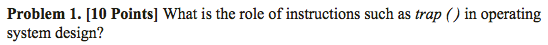
\includegraphics[width=14cm]{p1}
\end{center}
\end{figure}

When designing an operating system, you want to provide various operations to your
processes, such as printing and reading to files, that interact with the various
devices that the OS is controlling.  When a trap instruction is executed, a number
of things happen.  Most importantly, the kernel takes over control, and decides
whether or not to provide the requested servcie to the process.  A trap is also
used to catch errors.  If something happens to a process to make an exception, a
trap call is used so that the kernel can begin to handle it.

\begin{figure}[H]
\begin{center}
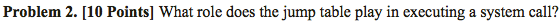
\includegraphics[width=14cm]{p2}
\end{center}
\end{figure}

Since there are 300+ syscalls, it is most efficient and easiest to call on an
array of function pointers with each syscall directly accesed using the ID
number of the syscall.  When the syscall is initiated, the kernel acceses this
table to find the relavant call code.

\begin{figure}[H]
\begin{center}
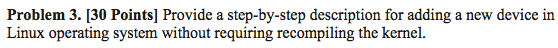
\includegraphics[width=14cm]{p3}
\end{center}
\end{figure}

In order to add a new device, the kernel itself needs to be changed, without
having to compile means that a loadable kernel module needs to be used. First,
create you C code to access the device.  Second, run insmod to add the module
to the running kernel.

\begin{figure}[H]
\begin{center}
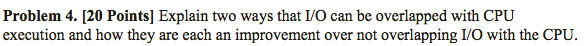
\includegraphics[width=14cm]{p4}
\end{center}
\end{figure}

One way is to have a seperate controller to access the I/O.  This allows the
second controller to read and buffer data from vaious devices while the CPU
does other work.  Then the CPU can read in all that data at once when the
device manager decides to interrupt.  This is faster since most CPU's are much
much faster than most devices.  If the CPU is waiting for the slow device, then
it is not being fully utilized.  The second method would be to use a polling
system.  Every now and then the CPU can stop execution of its main code to
check all of the devices to see if they have done anything.  This is good for
the same reason, it allows the CPU to do work in between checking for I/O.

\begin{figure}[H]
\begin{center}
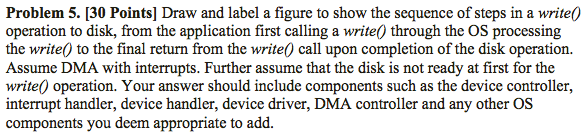
\includegraphics[width=14cm]{p5}
\end{center}
\end{figure}


\end{document}
